\chapter{Data Collection}

To support the creation of a student model we have collected our own data. We designed a paper test of mathematical knowledge of grammar school students. The test focused on simple functions (mostly polynomial, trigonometric, and exponential/logarithmic). Students were asked to solve various mathematical problems\footnote{In this case we use the term mathematical ``problem'' due to its nature. In general tests,	 terms ``question'' or ``item'' are often used. In this article all of these terms are interchangeable.} including graph drawing and reading, calculation of points on the graph, root finding, description of function shape and other function properties. 

\section{Test Design}
It is essential to note that this test is not meant for student school qualification and no grades which would influence student's school results were given.

The test design went through two rounds. First, we prepared an initial version of the test. This version was carried out by a small group of students and took about 80 minutes to be solved. We evaluated this first version and based on this evaluation we made changes before the main test cycle. It was necessary to limit the time of the test to 45 minutes to make it fit to one school lesson. Some problems were removed completely from the test. They were mainly those where the information benefit of the problem was too low due to its high or low difficulty (i.e. only a few students answered them correctly or incorrectly). There was no assumption that all the students should be able to finish all the questions in time which is a usual way to create school tests. In this case we were targeting the number of questions to allow the best students to finish just in time. This allowed us to remove less questions than we normally would. Remaining problems were updated and changed to be better understandable.  Moreover we divided problems into subproblems in the way that: 
\begin{itemize}
\item[(a)] it is possible to separate the subproblem from the main problem and solve it independently or 
\item[(b)] it is not possible to separate the subproblem, but it represents a subroutine of the main problem solution. 
\end{itemize}
Note that each subproblem of the first type can be viewed as a completely separate problem. 
On the other hand, subproblems of the second type are inseparable pieces of a problem.\\

The final version of the test contains 29 mathematical problems. These problems have been further divided into 53 subproblems. Subproblems are graded so that the sum of their grades is the grade of the parent problem, i.e., it falls into the set $\{0,\ldots,4\}$. Usually a question is divided into two parts each graded by at most two points\footnote{There is one exception from this rule: The first problem is very simple and it is divided into 8 parts, each graded by zero or one point (summing to the total maximum of 8).}. The granularity of subproblems is not the same for all of them and is a subset of the set $\{0,\ldots,4\}$. All together, the maximal possible score to obtain in the test is 120 points. \\
In an alternative evaluation approach, each subproblem is evaluated using the Boolean values (correct/wrong). The answer is evaluated as correct only if the solution of the subproblem and the solution method is correct unless there is an obvious numerical mistake. 

We organized tests at four grammar schools. In total 281 students participated in testing. In addition to answers to problems, information about students was collected. This includes mostly some personal factors as sex, age, and grades from mathematics, physics, and chemistry from the recent period. These factors will be used to better differentiate between students and to better predict their performance as well as to verify the validity of the test. We remind again that the goal of the tests was not the student evaluation. The goal was to provide them with valuable information about their weak and strong points. Students are able to view their result (the scores obtained in each individual problem) as well as a comparison with the rest of the test group. The comparisons were provided in the form of quantiles in the group of their class, school, and all participants.

\section{Test Assessment}
In the following section we present a psychometric analysis of the test. This kind of analysis should be done for every large scale test. It might not be necessary to perform all actions which are presented below for CAT. Nevertheless we will use these results to compare classical approach and CAT as well as to point out some interesting relations. Moreover it proves that the paper test we used to collect data provide reasonable results.

\textbf{True scores and reliability}\\
The goal of every test is to measure a certain variable. This variable reflects examinee's skill, ability or level of another quality (some psychiatric test might be measuring person's empathy). In terms of IRT and CAT this variable is a part of the student model described in the section~\ref{sec_IRT}. Even in the classical test there is a certain variable. A test is just a tool created to measure this variable. As always, when measuring anything, the measurement process is obstructed with measurement errors. These errors are caused by many different factors (the examinee could have a bad day, be ill, guess the answer, or get distracted while solving a single problem,\ldots) and it is reasonable to expect them to have a significant influence on the final value. The value obtained as a measurement $x$ of the variable $X$ is called a raw score and is in the form
$$x = \tau + e$$
where $\tau$ is the true score and $e$ is an additive error. 

There is an obvious question whether the raw score is influenced more by the true score or the error. For many measurements the maximum-likelihood estimator of the error is the variance of many consecutive measurements of the same factor. In our case it proves to be impractical to measure one person multiple times for obvious reasons. It is not as well possible to use the variance of many different examinees as their true values most likely differ. The variability of scores in the data set is then caused by actual differences between examinees (different true scores) as well as errors. It is usually expected that the data set satisfies homoskedasticity condition\footnote{Homoskedasticity means that the size of an error is not correlated with the size of the measured variable}. With this assumption true scores and errors are statistically independent and thus the observed variance $\sigma_x$ is a sum of variances of true scores $\sigma_\tau$ and errors $\sigma_e$.
$$\sigma_x=\sigma_\tau+\sigma_e$$
The best possible situation is that the variance of the measured variable X is fully modeled by true scores. This situation is very unlikely to happen. To determine the level of the relationship we use the value called reliability\footnote{Note that reliability is a well established and very important property of a test among psychometric society} which is defined as follows:
$$r_{xx} = \frac{\sigma_\tau}{\sigma_x}=\frac{\sigma_\tau}{\sigma_\tau+\sigma_e}$$
The higher the value the better. Unfortunately variables $\sigma_\tau$ in the nominator as well as $\sigma_e$ in the denominator of the second fraction are hidden (unobservable) variables and as such we are unable to evaluate their variance. The reliability has to be estimated with a different approach. 

There are many possible approaches and we will elaborate more into one of them which is known as Cronbach’s alpha coefficient. The idea is that items of the test are measuring the same factor and thus they should correlate with each other. The amount of pair wise correlations for $q$ questions is ${k=\frac{q(q-1)}{2}}$. All these correlations are put together in the Cronbach’s alpha coefficient which can be calculated as
$$r_{xx}\approx\alpha=\frac{n}{n-1}\left(1-\frac{\sum_{i=1}^{n}\sigma_i^2}{\sigma_t^2}\right)$$
where $\sigma_i$ is the variance of the ith item of the test, $\sigma_t$ is the variance of the whole test and $n$ is the number of items in the test. The coefficient should reach high values. According to \cite{1964psychometrics} any value below 0.5 means the test is of no use. Quality results are produced with the coefficient over 0.9.

For our data set (281 students) the following values were calculated:\\
Cronbach’s alpha for the numeric classification: $\alpha = 0.914$\\
Cronbach’s alpha for the Boolean classification: $\alpha = 0.925$\\
These values show reasonably high reliability of the test.

\textbf{Normalization and standard scores}\\
It may not be very efficient to use directly the score a student obtained in the test. This score is called the raw score. The problem with raw score is that it may not distinguish between individual students as well as it could. For example in case we have 3 results with scores of 20, 40 and 60 respectively. It would seem to us that the gap between the first and the second pair is the same. It definitely is in terms of raw score, but it may not be in terms of real abilities of students. If there are a lot of students who score between 20 and 40 and just a few in the interval between 40 and 60 then the skill gap from the second to the third may not be as wide as it appears. In order to better categorize students, scores are usually normalized. With normalized scores it is easier to evaluate the position of a student in the test for a specialist who is used to work with normalized scores. There are many different types of standard scores and most of them are obtained by a linear transformation of raw scores (note that it means that the order of examinees is not changed by this kind of transformation) by the following formula
$$x'=\mu'+\sigma'\frac{(x-\mu)}{\sigma}$$  
Where $x'$ is the transformed score, $\mu'$ and $\sigma'$ are desired mean and variance values of the standardized score, $\mu$ and $\sigma$ are previous mean and variance values and $x$ is the raw score. 

To apply these transformations it is required that the raw score belong to the Gaussian distribution (ideally with the mean value in the middle of possible scores). Standardized scores differ in the chosen parameters of $\mu'$ and $\sigma'$ and some special selections are generally recognized. The most commonly used is the z-score with the mean value~0 and the variance~1. Another well known standard score is the IQ~score (${\mu' = 100}$, ${\sigma'=15}$) used mostly for intelligence testing. Other well known scores are also stens, stenines, percentiles, and t-scores.

The set of scores obtained from our data set most likely do not belong to Gaussian distribution. The visual proof is displayed in the Figure~\ref{pic:gauss} where it can be clearly seen that it does not resemble the Gaussian distribution. The Shapiro-Wilk normality test also rejects the null hypothesis of the Gaussian distribution by resulting with $p-value = 3.648\cdot^{-7}$. The solution to this problem is provided by the McCall’s [McCall, W. A. (1922). How to measure in education. New York, NY: Macmillan] area standardization~\cite{2011psychometrics} which transforms raw scores to the Gaussian distribution. We performed this step at first and then we transformed scores to the standardized score scales. To illustrate these scales, a short excerpt from whole scale tables for the z-score and the IQ score is shown in the Table~\ref{tab:scores}. From this table we can see that the center of the normalized score scale is around 40 points of raw score (z value of 0 and IQ of 100). Maximum score obtained was 107 points and minimum 0. The transformed scale at these points has opposite (and extreme) values. The space between center of 40 points and these extremes is the same at both sides for normalized scores but it is not for raw scores. There is the same amount of students scoring in any two intervals of the same length ending/starting at the center on the normalized score scale (for example the same amount of students scored in intervals (-1,0) and (0,1) on the z-score, which corresponds to raw scores of (20, 40) and (40, 72 - not in the table)).


\begin{figure}%
\begin{center}
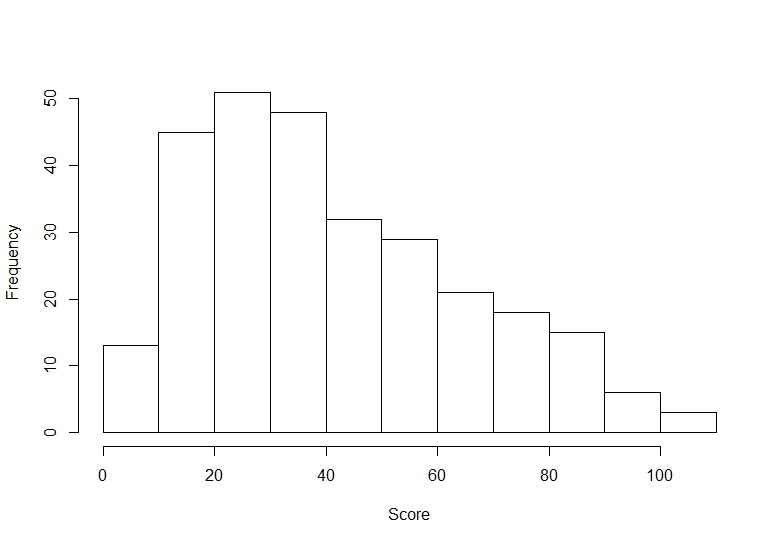
\includegraphics[width=9.5cm]{obr/histogram.png}%
\caption{Score frequency}%
\label{pic:gauss}%
\end{center}
\end{figure}


% Table generated by Excel2LaTeX from sheet 'List1'
\begin{table}[htbp]
  \centering
  \caption{Standardized scores}
	\label{tab:scores}
    \begin{tabular}{lrrrrrrr}
		\hline
    raw&0&20&40&60&80&100&107\\
    \hline
    z&-2.91&-1.00&-0.01&0.67&1.16&2.06&2.91\\
    IQ&56&85&100&110&117&131&144\\
    \hline
    \end{tabular}%
  \label{tab:addlabel}%
\end{table}%


\textbf{Validity}\\
Another question it is important to ask is whether the test is actually measuring the factor it is supposed to measure (i.e. in our case if the score obtained reflects mathematical skills rather than for example the ability to read the question or the writing skill of the examinee). This characteristic is called validity and there are many different ways of proving the test is valid. Most validity proofs come from the outside of the test. One way is to let an examinee to answer a new different test measuring the same factor (ideally a test which is already well established). Another way is to consult other factors known about the examinee, which is what was performed in our case.

As was mentioned above, in addition to solutions to individual problems student's grades from subjects (mathematics, physics, and chemistry) were obtained. It is reasonable to expect a correlation between these grades and the score reached. The correlation is present and its values are shown in the following paragraphs. Because of this fact, although the complete validation would require more thorough examination, it is expected that the test is valid.

\section{Preliminary Test Statistics}
In this section we present an overview of results obtained in testing. This should provide an idea of skills of students, prove validity as mentioned in the paragraph above and will also be referenced later on for comparison.



\begin{table}[htbp]
  \centering
  \caption{Average test scores of the four grammar schools.}
	
	\vspace{3mm}
	
    \begin{tabular}{l|rrrr|r|}
		\hline
    &\textbf{GS1}   & \textbf{GS2} & \textbf{GS3} & \textbf{GS4} & \textbf{Total} \\
					\hline
    &42.76 & 46.68 & 46.35 & 43.65 & 44.53 \\
    \textbf{Males} & 51.40  & 40.08 & 47.77 & 51.03 & 48.48 \\
    \textbf{Females} & 42.53 & 54.86 & 44.45 & 38.81 & 43.06 \\
		\hline
    \end{tabular}%
  \label{tab:totals}%
\end{table}%

The Table~\ref{tab:totals} shows the reached scores divided by gender and school. We calculated Pearson's correlation coefficients of score with other factors. Results are shown in the Table~\ref{tab:corr1}. The correlation test is associated with its p-value, where the null hypothesis is correlation of 0 (no correlation). It means we can say that the correlation between score and all grades (math, physics, and chemistry) is present. The negative value of correlation means that better grade (lower value) yields better score (higher value) which is expected. Furthermore we can see that the grade in mathematics has the highest correlation while physics and chemistry lower. Another significant correlation is interestingly between the fact that the student filled his/her name and his/her score. Positive value shows that those students who filled their name scored better in the test.
On the other hand we can not reject the null hypothesis for gender, so there most likely is no statistically significant correlation between gender and score\footnote{Females were encoded as 1 and males as -1. Negative value would show worst score for females, but it is statistically insignificant.}.

\begin{table}[htbp]%
\caption{Correlations of the score with other factors}
\label{tab:corr1}
\begin{center}
    \begin{tabular}{rrrrrr}
    \hline
    \multicolumn{1}{l}{\textbf{}}  & \multicolumn{1}{l}{\textbf{Gender}} & \multicolumn{1}{l}{\textbf{Mathematics}} & \multicolumn{1}{l}{\textbf{Physics}} & \multicolumn{1}{l}{\textbf{Chemistry}}& \multicolumn{1}{l}{\textbf{Name}} \\
    \hline
    \textbf{Correlation}&  -0.10  & -0.59  & -0.42  & -0.41  & 0.22\\
		\textbf{p-value}&  0.08  & $2.20e^{-16}$  & $3.63e^{-12}$  & $2.65e^{-11}$ & $0.18e^{-4}$ \\
    \hline
    \end{tabular}%
\end{center}
\end{table}

Some questions were in the form of real life problems rather than mathematical problems. These questions were correlated with the score independently as well. The result is displayed in the Table~\ref{tab:corr2}. In the first column it is possible to see that there is a strong and statistically significant correlation of the score obtained in these questions with the total score. Also in this case there is not a strong correlation with the sex of the student even though a bit higher and on the edge of rejection of statistical insignificance. The trend of correlations with grades is preserved but the strength of correlation is lower. In connection with previous results, it leads to an assumption that students with worse grades from these subjects answered correctly rather this kind of questions than other questions.

\begin{table}[htbp]%
\caption{Correlations of the real life problems with other factors}
\label{tab:corr2}
\begin{center}
    \begin{tabular}{rrrrrr}
    \hline
    \multicolumn{1}{l}{\textbf{}} & \multicolumn{1}{l}{\textbf{Score}} & \multicolumn{1}{l}{\textbf{Gender}} & \multicolumn{1}{l}{\textbf{Mathematics}} & \multicolumn{1}{l}{\textbf{Physics}} & \multicolumn{1}{l}{\textbf{Chemistry}} \\
    \hline
    \textbf{Correlation}& 0.69  & -0.19  & -0.38  & -0.25  & -0.27  \\
		\textbf{p-value}& $2.20e^{-16}$   & $0.16e^{-3}$  & $3.16e^{-10}$  & $7.99e^{-5}$   & $2.25e^{-5}$   \\
    \hline
    \end{tabular}%
\end{center}
\end{table}
